\documentclass[12pt]{article}
\usepackage[a4paper, margin=0.75in]{geometry}
\usepackage[document]{ragged2e}
\usepackage{graphicx}
\usepackage{subcaption}
\graphicspath{ {./images/} }
\usepackage{enumerate}
\usepackage{framed}
\usepackage{amsmath,amsfonts,amsthm,thmtools,amssymb,mathtools,commath}
\usepackage{physics}
\usepackage{tikz}
\usetikzlibrary{mindmap}
\usepackage{caption}
\usepackage{xcolor}
\usepackage[most]{tcolorbox}
\usepackage{cleveref}


%%%%%%%%%%%%%%%%
%  Definition  %
%%%%%%%%%%%%%%%%
\tcbuselibrary{theorems,skins,hooks}
\newtcbtheorem[number within=subsection]{definition}{Definition}%
{
    % theorem style=definition,
    enhanced,
	before skip=2mm,after skip=2mm, colback=cyan!5,colframe=cyan!80!black,boxrule=0.5mm,
	attach boxed title to top left={xshift=1cm,yshift*=1mm-\tcboxedtitleheight},
	boxed title style={frame code={
					\path[fill=cyan]
					([yshift=-1mm,xshift=-1mm]frame.north west)
					arc[start angle=0,end angle=180,radius=1mm]
					([yshift=-1mm,xshift=1mm]frame.north east)
					arc[start angle=180,end angle=0,radius=1mm];
					\path[left color=cyan!30!black,right color=cyan!30!black,
						middle color=cyan!50!black]
					([xshift=-2mm]frame.north west) -- ([xshift=2mm]frame.north east)
					[rounded corners=1mm]-- ([xshift=1mm,yshift=-1mm]frame.north east)
					-- (frame.south east) -- (frame.south west)
					-- ([xshift=-1mm,yshift=-1mm]frame.north west)
					[sharp corners]-- cycle;
				},interior engine=empty,
		},
	fonttitle=\bfseries,
	title={#2},#1
}{def}


%%%%%%%%%%%%%
%  Theorem  %
%%%%%%%%%%%%%
\tcbuselibrary{theorems,skins,hooks}
\newtcbtheorem[use counter from=definition]{theorem}{Theorem}%
{
    theorem style=plain,
    enhanced,
    colframe=green,
    boxrule=1pt,
    titlerule=0mm,
    toptitle=1mm,
    bottomtitle=1mm,
    fonttitle=\bfseries,
    fontupper=\mdseries\itshape,
    coltitle=green!30!black,
    colbacktitle=cyan!15!white,
    colback=green!10,
    description font=\bfseries\sffamily
}{thrm}


%%%%%%%%%%%%%%
% Corollary  %
%%%%%%%%%%%%%%
 \tcbuselibrary{theorems,skins}
 \newtcbtheorem[use counter from=theorem]{corollary}{Corollary}%
 {
    theorem style=plain,
    enhanced,
    colframe=green,
    frame hidden,
    titlerule=0mm,
    toptitle=1mm,
    bottomtitle=1mm,
    fonttitle=\bfseries,
    fontupper=\mdseries\itshape,
    coltitle=green!30!black,
    colbacktitle=cyan!15!white,
    colback=green!10,
    description font=\bfseries\sffamily
 }{corl}


%%%%%%%%%%%%%
%  Example  %
%%%%%%%%%%%%%
\tcbuselibrary{theorems,skins,hooks}
\newtcbtheorem[number within=section]{example}{Example}%
{
	enhanced,
	breakable,
	colback = gray!5,
	frame hidden,
	boxrule = 0sp,
	borderline west = {2pt}{0pt}{gray},
	sharp corners,
	detach title,
	before upper = \tcbtitle\par\smallskip,
    coltitle=gray!70!black,
	fonttitle = \bfseries\sffamily,
	description font = \mdseries\bfseries
}
{xmp}


%%%%%%%%%%%%%%
%  Exercise  %
%%%%%%%%%%%%%%
\tcbuselibrary{theorems,skins,hooks}
\newtcbtheorem[number within=section]{exercise}{Exercise}%
{
    enhanced,
    breakable,
    colback=black!5,
    colframe=black!30,
    left=0.5em,
    before skip=10pt,
    after skip=10pt,
    boxrule=0pt,
    boxsep=0pt,
    arc=0pt,
    outer arc=0pt,
    borderline west={3pt}{0pt}{black!30},
}{exc}

%%%%%%%%%%
%  Note  %
%%%%%%%%%%
\usetikzlibrary{arrows,calc,shadows.blur}
\tcbuselibrary{skins}
\newtcolorbox{note}[1][]{%
	enhanced jigsaw,
	colback=gray!20!white,%
	colframe=gray!80!black,
	size=small,
	boxrule=1pt,
	title=\textbf{Note:-},
	halign title=flush center,
	coltitle=black,
	breakable,
	drop shadow=black!50!white,
	attach boxed title to top left={xshift=1cm,yshift=-\tcboxedtitleheight/2,yshifttext=-\tcboxedtitleheight/2},
	minipage boxed title=1.5cm,
	boxed title style={%
			colback=white,
			size=fbox,
			boxrule=1pt,
			boxsep=2pt,
			underlay={%
					\coordinate (dotA) at ($(interior.west) + (-0.5pt,0)$);
					\coordinate (dotB) at ($(interior.east) + (0.5pt,0)$);
					\begin{scope}
						\clip (interior.north west) rectangle ([xshift=3ex]interior.east);
						\filldraw [white, blur shadow={shadow opacity=60, shadow yshift=-.75ex}, rounded corners=2pt] (interior.north west) rectangle (interior.south east);
					\end{scope}
					\begin{scope}[gray!80!black]
						\fill (dotA) circle (2pt);
						\fill (dotB) circle (2pt);
					\end{scope}
				},
		},
	#1,
}


\title{
    Experiment 2\\
    \textbf{Output Characteristics Analysis of Fixed Bias and Voltage Divider Bias}
}

\author{
    Turja Roy\\
    2108052
}
\date{January 22, 2024}

\begin{document}
\maketitle

\section{Objective}
\begin{enumerate}
    \item To determine the output characteristics of fixed bias configuration
    \item To determine the output characteristics of voltage divider bias configuration
\end{enumerate}

\section{Apparatus}
\begin{enumerate}
    \item Transistor (2N3904 n-p-n)
    \item Resistors ($10k\Omega$, $1k\Omega$, $650\Omega$, $560\Omega$)
    \item Multimeter
    \item Ammeters (mA and $\mu$A)
    \item Breadboard
    \item Wires
    \item DC Power Supply (0-30V)
\end{enumerate}

\section{Circuit Diagram}
\begin{figure}[h!]
    \centering
    \begin{subfigure}{0.45\textwidth}
        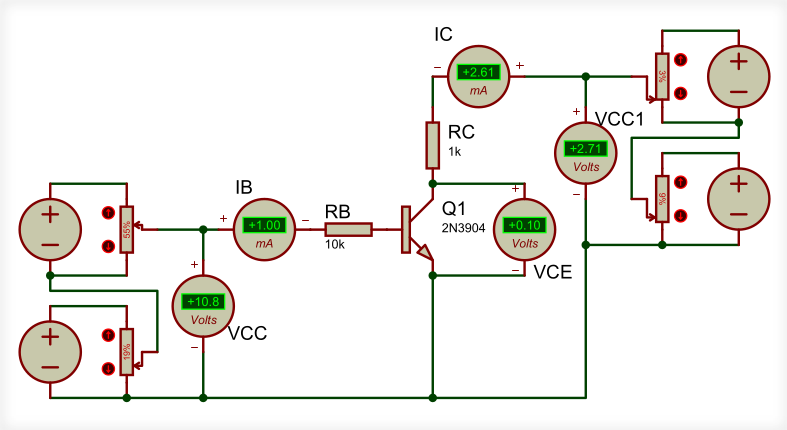
\includegraphics[width=0.9\linewidth]{Fixed_Bias.png}
        \caption{Fixed Bias Configuration}
    \end{subfigure}
    \begin{subfigure}{0.45\textwidth}
        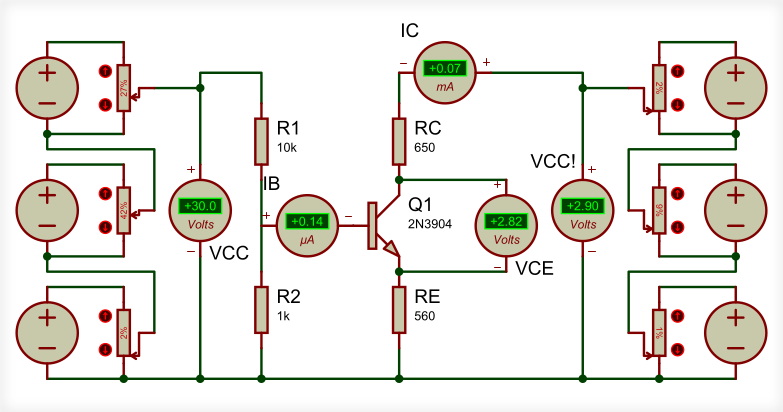
\includegraphics[width=0.9\linewidth]{Voltage_Divider_Bias.png}
        \caption{Voltage Divider Bias Configuration}
    \end{subfigure}
    \caption{Circuit Diagrams}
\end{figure}

\newpage
\section{Data Analysis}
\subsection{Theoretical Data}

\subsubsection{Fixed Bias Configuration}
\bgroup
\def\arraystretch{1.5}
\begin{table}[h!]
    \centering
    \begin{tabular}{|c|c|c||c|c|c|}
        \hline
        \multicolumn{3}{|c||}{$I_B = 0 \mu A$} & \multicolumn{3}{|c|}{$I_B = 11 \mu A$} \\
        \hline
        $V_{CC}$ (V) & $V_{CE}$ (V) & $I_C$ (mA) & $V_{CC}$ (V) & $V_{CE}$ (V) & $I_C$ (mA) \\ \hline
        2.7 & 2.7 & 0.0 & 0.0 & 0.0 & 0.0 \\
        5.7 & 5.7 & 0.0 & 2.7 & 1.6 & 1.1 \\
        9.0 & 9.0 & 0.0 & 5.6 & 4.5 & 1.1 \\
        11.1 & 11.1 & 0.0 & 9.0 & 7.9 & 1.1 \\
        15.0 & 15.0 & 0.0 & 12.0 & 10.9 & 1.1 \\
        18.0 & 18.0 & 0.0 & 15.3 & 14.2 & 1.1 \\
        21.9 & 21.9 & 0.0 & 18.4 & 17.3 & 1.1 \\
        25.2 & 25.2 & 0.0 & 21.8 & 20.7 & 1.1 \\
        28.0 & 28.0 & 0.0 & 25.2 & 24.1 & 1.1 \\
        \hline
    \end{tabular}
    \caption{caption}
    \label{Theoretical Fixed Bias}
\end{table}
\egroup
\vspace{-20pt}
\[
    I_C = \beta I_B
\] \[
    V_{CE} = V_{CC} - I_C R_C
\]

\subsubsection{Voltage Divider Bias Configuration}
\bgroup
\def\arraystretch{1.5}
\begin{table}[h!]
    \centering
    \begin{tabular}{|c|c|c||c|c|c|}
        \hline
        \multicolumn{3}{|c||}{$I_B = 0 \mu A$} & \multicolumn{3}{|c|}{$I_B = 0.14 \mu A$} \\
        \hline
        $V_{CC}$ (V) & $V_{CE}$ (V) & $I_C$ (mA) & $V_{CC}$ (V) & $V_{CE}$ (V) & $I_C$ (mA) \\ \hline
        0.0 & 0.0 & 0.0 & 0.0 & 0.0 & 0.0 \\
        3.0 & 3.0 & 0.0 & 3.0 & 2.9831 & 0.014 \\
        8.0 & 8.0 & 0.0 & 8.0 & 7.9831 & 0.014 \\
        10.0 & 10.0 & 0.0 & 10.7 & 10.683 & 0.014 \\
        14.0 & 14.0 & 0.0 & 14.7 & 14.683 & 0.014 \\
        17.0 & 17.0 & 0.0 & 17.7 & 17.683 & 0.014 \\
        20.0 & 20.0 & 0.0 & 20.7 & 20.683 & 0.014 \\
        24.0 & 24.0 & 0.0 & 24.7 & 24.683 & 0.014 \\
        27.0 & 27.0 & 0.0 & 27.6 & 27.583 & 0.014 \\
        \hline
    \end{tabular}
    \caption{caption}
    \label{Theoretical Voltage Divider Bias}
\end{table}
\egroup
\vspace{-20pt}
\[
    I_C = \beta I_B
\] \[
    V_{CE} = V_{CC} - I_C (R_C + R_E)
\]

\subsection{Simulation Data and Practical Data}
\subsubsection{Fixed Bias Configuration}
\bgroup
\def\arraystretch{1.5}
\begin{table}[h!]
    \centering
    \begin{tabular}{|c|c|c||c|c|c||c|c|}
        \hline
        \multicolumn{3}{|c||}{\textbf{Simulation Data}} & \multicolumn{3}{|c||}{\textbf{Practical Data}} & \multicolumn{2}{|c|}{\textbf{Errors}} \\ \hline\hline
        \multicolumn{8}{|c|}{\textbf{$I_B = 0\mu A$}} \\ \hline
        $V_{CC}$ (V) & $V_{CE}$ (V) & $I_C$ (mA) & $V_{CC}$ (V) & $V_{CE}$ (V) & $I_C$ (mA) & \%$V_{CE}$ & \%$I_C$ \\ \hline
        0 & 0 & 0 & 0 & 0 & 0 & 0 & 0 \\
        2.7 & 2.7 & 0 & 2.7 & 2.02 & 0 & 25.19 & 0  \\
        5.6 & 5.6 & 0 & 5.6 & 5.01 & 0 & 10.54 & 0 \\
        9 & 9 & 0 & 9 & 8.16 & 0 & 9.33 & 0 \\
        12 & 12 & 0 & 12 & 10.5 & 0 & 12.5 & 0 \\
        15.3 & 15.3 & 0 & 15.3 & 13.9 & 0 & 9.15 & 0 \\
        18.4 & 18.4 & 0 & 18.4 & 17.5 & 0 & 4.89 & 0 \\
        21.8 & 21.8 & 0 & 21.8 & 21.27 & 0 & 2.43 & 0 \\
        25.2 & 25.2 & 0 & 25.2 & 24.3 & 0 & 3.57 & 0 \\
        28.2 & 28.2 & 0 & 28.2 & 27.2 & 0 & 3.55 & 0 \\ \hline\hline
        \multicolumn{8}{|c|}{\textbf{$I_B = 11\mu A$}} \\ \hline
        $V_{CC}$ (V) & $V_{CE}$ (V) & $I_C$ (mA) & $V_{CC}$ (V) & $V_{CE}$ (V) & $I_C$ (mA) & \%$V_{CE}$ & \%$I_C$ \\ \hline
        0 & 0 & 0 & 0 & 0 & 0 & 0 & 0 \\
        2.73 & 1.86 & 0.86 & 2.7 & 1.56 & 1 & 16.13 & 16.28 \\
        5.65 & 4.74 & 0.91 & 5.6 & 4.2 & 1 & 11.39 & 9.89 \\
        8.98 & 8.01 & 0.97 & 9 & 7.33 & 1 & 8.49 & 3.09 \\
        11.9 & 10.9 & 1.02 & 12 & 10.01 & 1 & 8.17 & 1.96 \\
        15.3 & 14.2 & 1.08 & 15.3 & 13.69 & 1 & 3.59 & 7.41 \\
        18.4 & 17.2 & 1.13 & 18.4 & 16.63 & 1.1 & 3.31 & 2.65 \\
        21.8 & 20.6 & 1.19 & 21.8 & 20.1 & 1.2 & 2.43 & 0.84 \\
        25.2 & 24 & 1.25 & 25.2 & 23.07 & 1.2 & 3.88 & 4 \\
        28.2 & 26.9 & 1.3 & 28.2 & 25 & 1.2 & 7.06 & 7.69 \\ \hline
    \end{tabular}
    \caption{Data Analysis for Fixed Bias Configuration}
    \label{Fixed Bias}
\end{table}
\egroup

\newpage
\subsubsection{Voltage Divider Bias Configuration}
\bgroup
\def\arraystretch{1.5}
\begin{table}[h!]
    \centering
    \begin{tabular}{|c|c|c||c|c|c||c|c|}
        \hline
        \multicolumn{3}{|c||}{\textbf{Simulation Data}} & \multicolumn{3}{|c||}{\textbf{Practical Data}} & \multicolumn{2}{|c|}{\textbf{Errors}} \\ \hline\hline
        \multicolumn{8}{|c|}{\textbf{$I_B = 0\mu A$}} \\ \hline
        $V_{CC}$ (V) & $V_{CE}$ (V) & $I_C$ (mA) & $V_{CC}$ (V) & $V_{CE}$ (V) & $I_C$ (mA) & \%$V_{CE}$ & \%$I_C$ \\ \hline
        0 & 0 & 0 & 0 & 0 & 0 & 0 & 0 \\
        3 & 3 & 0 & 3 & 2.7 & 0 & 10 & 0 \\
        8 & 8 & 0 & 8 & 7.6 & 0 & 5 & 0 \\
        10 & 10 & 0 & 10 & 9.3 & 0 & 7 & 0 \\
        14 & 14 & 0 & 14 & 13.87 & 0 & 0.93 & 0 \\
        17 & 17 & 0 & 17 & 16.4 & 0 & 3.53 & 0 \\
        20 & 20 & 0 & 20 & 19.1 & 0 & 4.5 & 0 \\
        24 & 24 & 0 & 24 & 23.6 & 0 & 1.67 & 0 \\
        27 & 27 & 0 & 27 & 26.7 & 0 & 1.11 & 0 \\ \hline\hline
        \multicolumn{8}{|c|}{\textbf{$I_B = 0.14\mu A$}} \\ \hline
        $V_{CC}$ (V) & $V_{CE}$ (V) & $I_C$ (mA) & $V_{CC}$ (V) & $V_{CE}$ (V) & $I_C$ (mA) & \%$V_{CE}$ & \%$I_C$ \\ \hline
        0 & 0 & 0 & 0 & 0 & 0 & 0 & 0 \\
        3 & 2.91 & 0.07 & 3 & 2.91 & 0.07 & 3.09 & 90 \\
        8 & 7.9 & 0.08 & 8 & 7.9 & 0.07 & 1.27 & 88.57 \\
        10.7 & 10.6 & 0.09 & 10.7 & 10.6 & 0.07 & 0.94 & 87.14 \\
        14.7 & 14.5 & 0.1 & 14.7 & 14.5 & 0.11 & 1.38 & 10 \\
        17.7 & 17.5 & 0.11 & 17.7 & 17.5 & 0.11 & 1.14 & 0 \\
        20.7 & 20.5 & 0.12 & 20.7 & 20.5 & 0.11 & 0.98 & 8.33 \\
        24.7 & 24.5 & 0.13 & 24.7 & 24.5 & 0.11 & 0.82 & 15.38 \\
        27.6 & 27.5 & 0.14 & 27.6 & 27.5 & 0.11 & 0.36 & 21.43 \\ \hline
    \end{tabular}
    \caption{Data Analysis for Voltage Divider Bias Configuration}
    \label{Voltage Divider Bias}
\end{table}

\newpage

\section{Graphs}
\begin{figure}[h!]
    \centering
    \begin{subfigure}{0.49\textwidth}
        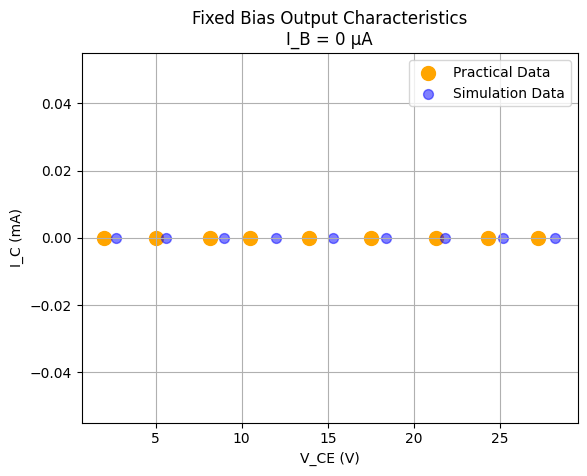
\includegraphics[width=0.9\linewidth]{FB_0A.png}
        \caption{$I_B = 0\mu A$}
    \end{subfigure}
    \begin{subfigure}{0.49\textwidth}
        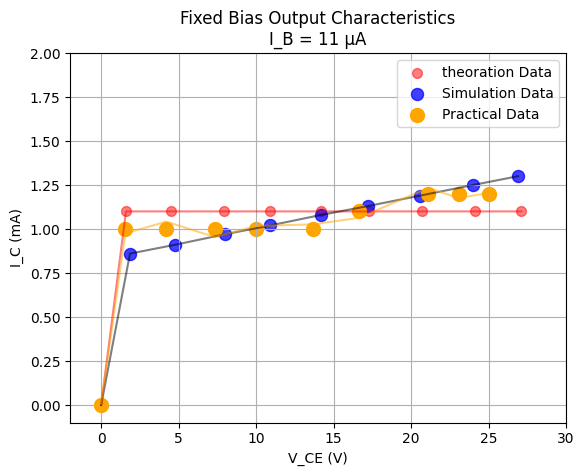
\includegraphics[width=0.9\linewidth]{FB_11A.png}
        \caption{$I_B = 11\mu A$}
    \end{subfigure}
    \caption{Output Characteristics of Fixed Bias Configuration}
    \label{Fixed Bias Graph}
\end{figure}

\begin{figure}[h!]
    \centering
    \begin{subfigure}{0.49\textwidth}
        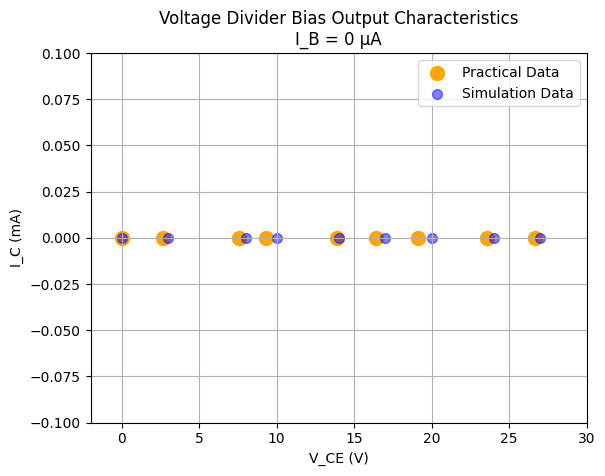
\includegraphics[width=0.9\linewidth]{VD_0A.png}
        \caption{$I_B = 0\mu A$}
    \end{subfigure}
    \begin{subfigure}{0.49\textwidth}
        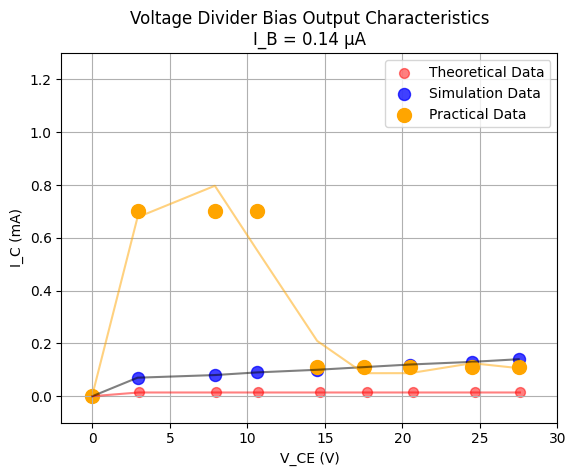
\includegraphics[width=0.9\linewidth]{VD_0.14A.png}
        \caption{$I_B = 0.14\mu A$}
    \end{subfigure}
    \caption{Output Characteristics of Voltage Divider Bias Configuration}
    \label{Voltage Divider Bias Graph}
\end{figure}

From the graphs, we can see that the theoretical data, the simulation, and the practical data are not exactly equal. This is due to some technical errors and precision errors. From the graph, a connecting line drawn between $V_{CE} = 0$ and $I_C = 0$ will intersect the output characteristic plot at a point called the Q-point or operational point. This Q-point can be modified by varying the values of $V_{CC}$ and $R_C$.

\newpage
\section{Discussion}
\begin{enumerate}[(a)]
    \item The experiment was conducted to learn about the biasing of transistors. Two biasings were analyzed: fixed bias, and voltage divider bias.
    \item All the biases were made using a 2N3904 n-p-n transistor in a common-emitter configuration.
    \item The output characteristics of the two biasing configurations were plotted and analyzed.
    \item The output characteristic graphs for simulation and practical data were plotted and compared.
    \item Error of the practical data from the simulation data was calculated.
    \item The errors were considered to happen due to technical errors and precision errors.
    \item More accurate equipment could be used to reduce the errors.
\end{enumerate}

\end{document}
